\documentclass[addpoints]{exam}

\makeatletter % Lagfæring fyrir nýjar útgáfur af TeXLive
\expandafter\providecommand\expandafter*\csname ver@framed.sty\endcsname
{2003/07/21 v0.8a Simulated by exam}
\makeatother

\usepackage[top=2cm, bottom=2cm, left=1.5cm, right=1.5cm]{geometry}
\usepackage[utf8]{inputenc}
\usepackage[icelandic]{babel}
\usepackage[T1]{fontenc}
%\usepackage[sc]{mathpazo}
\usepackage{helvet} \renewcommand\familydefault{\sfdefault}
\usepackage[parfill]{parskip}
\usepackage{tabularx}
\usepackage{multirow}
\usepackage{multicol}
\usepackage{graphicx}
\usepackage{enumerate}
\usepackage{amsmath, amsfonts, amssymb, amsthm}
\usepackage{minted} %Minted and configuration
\usepackage{afterpage}
\usepackage{scrextend}

\usepackage[pdftex,bookmarks=true,colorlinks=true,pdfauthor={Eirikur Ernir Thorsteinsson},linkcolor=blue,urlcolor=blue]{hyperref}

\setcounter{secnumdepth}{-1} 
\hyphenpenalty=5000

\hyphenation{non-deterministic auto-maton auto-matons}

\newcommand\blankpage{%
    \null
    \thispagestyle{empty}%
    \addtocounter{page}{-1}%
    }

\usemintedstyle{default}
\renewcommand{\theFancyVerbLine}{\sffamily \arabic{FancyVerbLine}}
\author{}
\date{}

\footer{}{}{}

\setcounter{secnumdepth}{-1} 

\qformat{\large \textbf Spurning \thequestion \phantom{M}(\totalpoints \phantom{l}stig) \hfill}
\renewcommand{\solutiontitle}{\noindent\textbf{Svar:}\par\noindent}
\renewcommand{\points}{stig}
\renewcommand{\questionshook}{\setlength{\itemsep}{0.5cm}}
\hqword{Spurning:}
\hpword{Stig í boði:}
\hsword{Stig:}
\htword{Samtals}

\title{TÖL104G Stærðfræðimynstur í tölvunarfræði - upptökupróf}
\author{}
\date{}

\pagestyle{headandfoot}
\firstpageheader{TÖL104G}{Upptökupróf//Secondary exam}{janúar 2018}
\firstpagefooter{}{Bls. \thepage\ af \numpages}{}
\runningfooter{}{Bls. \thepage\ af \numpages}{}
\setlength{\columnsep}{0.5cm}

\changefontsizes{14pt}

% \printanswers
\begin{document}

% \thispagestyle{empty}
Fullt nafn//Full name: \vspace*{1mm} \hrule

\begin{center}
    \begin{minipage}{\textwidth}
    
    \vspace{0.7cm}
    \paragraph{Leiðbeiningar} Á þessu prófi eru \numquestions\ spurningar sem samtals gefa \numpoints\ stig. Leyfileg hjálpargögn eru reiknivél og ein A4 blaðsíða af glósum.
    
    Heftið verður skannað inn í tölvu til yfirferðar. Vinsamlegast forðist ljósa blýanta, ekki rífa eða krumpa heftið og ekki bæta við blaðsíðum. 
    
    Til að svara krossaspurningum skal nota svartöfluna hér að neðan. Merkið vandlega við einn möguleika fyrir hverja spurningu. Ekki er dregið frá fyrir röng svör. 
    
    Til að svara almennum spurningum skal skrifa inn í svæðið sem fylgir strax á eftir hverri spurningu. Þurfi að koma viðbótarupplýsingum til skila skal skrifa það í rammana á öftustu blaðsíðunum. Aðrir hlutar heftisins, sér í lagi bakhliðar, \emph{verða ekki lesnir}.
    
    Dæmin á þessu prófi eru misþung. Þau eru ekki sett fram í erfiðleikaröð.
    
    \vspace{0.7cm}
    

    \begin{multicols}{2}

        \paragraph{Instructions} This exam consists of \numquestions\ questions worth a total of \numpoints\ points. You may bring a calculator and one A4 sheet of notes to the exam.
        
        This exam will be digitally scanned for grading. Please avoid light pencils, tearing or crumpling the pages and adding pages. 
        
        To answer multiple choice questions, use the answer table to the right. Carefully mark one option for each question. Points are not deducted for wrong choices. 
        
        To answer general questions, write within the area immediately following each question. If additional space is needed, write within the frames on the last two pages. Other parts of the exam sheets, particularly the overleaf, \emph{will not be read}.
        
        Some questions on this exam are less difficult than others, they are not ordered by difficulty.

        \begin{center}
            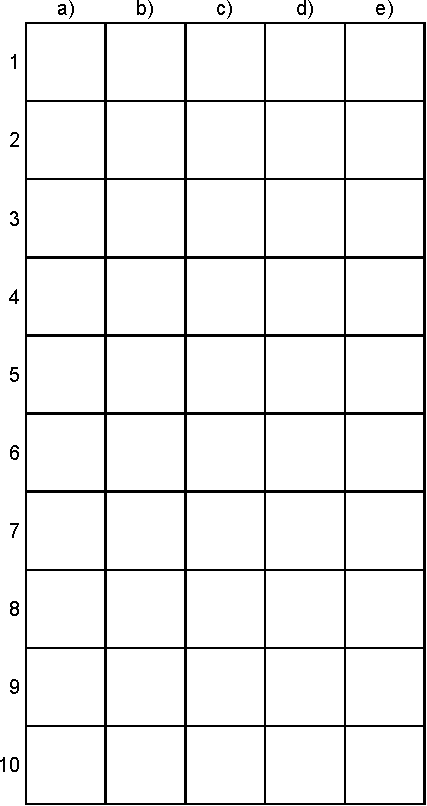
\includegraphics[width=0.7\linewidth]{Pics/svartafla}
        \end{center}
    \end{multicols}    
    \end{minipage}

\end{center}

\begin{questions}
        
\section{Krossaspurningar//Multiple Choice Questions}

\question[3] Hver eftirfarandi yrðinga er jafngild $\lnot  p \lor \lnot q$?

\begin{enumerate}[a)]
    \item $\lnot (p \oplus q)$
    \item $\lnot (p \lor q)$
    \item $\lnot (p \land q)$ % Rétt
    \item $(q \to p)$
    \item $(p \to q) \lor (q \to p)$
\end{enumerate}

\question[3] 

\textbf{(Ísl)} Hver eftirfarandi setninga er ekki framsetning á $p \to q$?

\textbf{(En)} Which of the following is not a way to express $p \to q$?

\begin{enumerate}[a)]
    \item Ef $p$, þá $q$ // if $p$, then $q$
    \item Nægjanlegt skilyrði fyrir $q$ er $p$ // a sufficient condition for $q$ is $p$
    \item $q$ þegar $p$ // $q$ whenever $p$
    \item $q$ nema $\lnot p$ // $q$ unless $\lnot p$
    \item Nauðsynlegt skilyrði fyrir $q$ er $p$ // a necessary condition for $q$ is $p$ % Rétt, þ.e.a.s. röng staðhæfing
\end{enumerate}

\question[3] 

\textbf{(Ísl)}  Hvað er $P(\{\emptyset,\{\emptyset\}\})$?

\textbf{(En)} What is $P(\{\emptyset,\{\emptyset\}\})$?

\begin{enumerate}[a)]
    \item $\{\emptyset,\{\emptyset\}\}$
    \item $\{\emptyset,\{\emptyset\}, \{\{\emptyset\}\}\}$
    \item $\phantom{\{}\emptyset$
    \item $\{\emptyset,\{\emptyset\}, \{\{\emptyset\}\}, \{\emptyset,\{\emptyset\}\}\}$ % Rétt
    \item $\{\{\emptyset\}, \{\{\emptyset\}\}, \{\emptyset,\{\emptyset\}\}\}$
\end{enumerate}

\question[3]

\textbf{(Ísl)} Hversu mörg spil þarf að velja úr hefðbundnum 52 spila stokki til að tryggja það að a.m.k. þrjú spil af sömu sort séu valin?

\textbf{(En)} How many cards must be selected from a standard deck of 52 cards to guarantee that at least three cards of the same suit are chosen?

\begin{tabularx}{\textwidth}{XXXXX} % d) Rétt
    a) 3 & b) 4 & c) 8 & d) 9 & e) 12 \\
\end{tabularx} 


\question[3] 

\textbf{(Ísl)} Á þessu prófi eru 10 krossaspurningar, hver þeirra er með 5 svarmöguleika. Á hve marga vegu er hægt að svara þessum krossum?

\textbf{(En)} This exam contains 10 multiple choice questions. Each of them has 5 choices. In how many ways can these questions be answered?

\begin{tabularx}{\textwidth}{XXXXX} % b) Rétt
    a) $10^5$& b) $5^{10}$& c) $10 \cdot 5!$& d) $10\cdot 5$& e) $5\cdot 10!$\\
\end{tabularx}

\question[3] 

\textbf{(Ísl)} Hver eftirfarandi vensla eru bæði samhverf og andsamhverf?

\textbf{(En)} Which of the following relations are both symmetric and antisymmetric?

\begin{enumerate}[a)]
    \item $\{(a, c), (c, b), (b, c), (c, a)\}$ á $\{a, b, c\}$
    \item $\{(a, b), (b, a)\}$ á $\{a,b\}$
    \item $\{(a, a), (a, b)\}$ á $\{a,b\}$
    \item $\{(a, a), (a, b), (b, a)\}$ á $\{a,b,c\}$
    \item Tómu venslin á $\{a\}$//The empty relation on $\{a\}$% Rétt
\end{enumerate}

\question[3] 

\textbf{(Ísl)} Samanhangandi lagnet hefur átta hnúta sem allir eru af stigi 3. Hve marga möskva hefur sléttunet þessa lagnets?

\textbf{(En)} A connected planar graph has eight vertices, each of degree 3. Into how many regions is the plane divided by a planar representation of this graph?

\begin{tabularx}{\textwidth}{XXXXX} %c rétt, e = (3*8)/2 = 12, r = 2 - v + e = 2 - 8 + 12 = 6.
    a) 2 & b) 4 & c) 6 & d) 8 & e) 12\\
\end{tabularx}

\question[3]

\begin{multicols}{2}
    \textbf{(Ísl)} Hvert er grennslafylki netsins til hliðar? Gerið ráð fyrir hnútaröðun í stafrófsröð.
    
    \textbf{(En)} Identify the adjacency matrix for the given graph Assume an alphabetic vertex order.

    \begin{center}
        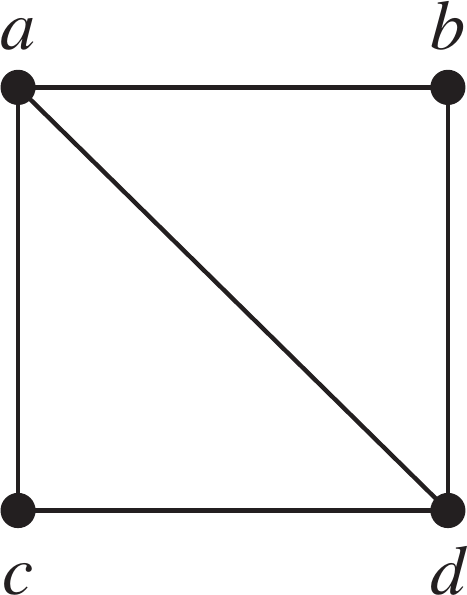
\includegraphics[width=0.33\linewidth]{Pics/exam-graph-tiny}
    \end{center}
\end{multicols}
\begin{center}
a)
$
\begin{bmatrix}
    1&0&0&0\\
    0&1&1&0\\
    0&1&1&0\\
    0&0&0&1\\
\end{bmatrix}    
$
b)
$
\begin{bmatrix}
    0&0&0&1\\
    0&1&1&0\\
    0&1&1&0\\
    1&0&0&0\\
\end{bmatrix}    
$
c)
$
\begin{bmatrix}
    1&1&1&0\\
    1&0&0&1\\
    1&0&0&1\\
    0&1&1&1\\
\end{bmatrix}    
$
d) % Rétt
$
\begin{bmatrix}
    0&1&1&1\\
    1&0&0&1\\
    1&0&0&1\\
    1&1&1&0\\
\end{bmatrix}    
$
e) 
$
\begin{bmatrix}
    1&1&1&1\\
    1&1&0&1\\
    1&0&1&1\\
    1&1&1&1\\
\end{bmatrix}    
$
\end{center}

\newpage

\question[3] 

\begin{multicols}{2}
    \textbf{(Ísl)} Gefið er rótartré. Hvert eftirfarandi er listi yfir hnúta þess í miðröð?
    
    \textbf{(En)} A rooted tree is given. Which of the following is an inorder listing of its vertices?

    \begin{enumerate}[a)]
        \item $a, b, d, e, f, g, c$ %Preorder
        \item $a, b, c, d, e, f, g$ %Stafrófsröð
        \item $c, a, g, e, f, b, d$
        \item $d, f, g, e, b, c, a$ %Postorder
        \item $d, b, f, e, g, a, c$ %Inorder, rétt
    \end{enumerate}
    \begin{center}
        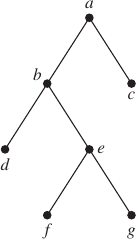
\includegraphics[width=0.5\linewidth]{Pics/exam-tree}
    \end{center}
\end{multicols}

\question[3]

\textbf{(Ísl)} Hvert af eftirfarandi á við um endanlega samþykkjara?

\textbf{(En)} Which of the following statements about finite-state automatons is correct?

\begin{enumerate}[a)]
    \item Sérhver briðggengur samþykkjari á sér jafngildan löggengan samþykkjara // Every nondeterministic automaton has an equivalent deterministic automaton % Rétt
    \item Til eru mál sem brigðgengir samþykkjarar geta samþykkt en löggengir ekki // Languages exist that can be recognized by nondeterministic automatons but not by deterministic automatons
    \item Brigðgengir samþykkjarar innihalda venjulega fleiri stöður en löggengir // Nondeterministic automatons generally have more states than deterministic automatons
    \item Hvert mál er samþykkt af nákvæmlega einum brigðgengum samþykkjara // Every language is recognized by precisely one nondeterministic automaton
    \item Í brigðgengum samþykkjara er færsla til nákvæmlega einnar stöðu skilgreind fyrir hvert par af stöðu og inntakstákni // A nondeterministic automaton maps every state-input pair to precisely one state
\end{enumerate}

\newpage
\section{Almennar spurningar//General Questions}

\question[10]

\textbf{(Ísl)} Látum $p, q$ og $r$ vera eftirfarandi yrðingar:

\begin{itemize}
    \item[] $p$: Birnir hafa sést nálægt stígnum
    \item[] $q$: Öruggt er að ganga eftir stígnum
    \item[] $r$: Ber vaxa meðfram stígnum
\end{itemize}

Setjið eftirfarandi yrðingar fram með því að nota $p, q$ og $r$ ásamt rökvirkjum:

\begin{enumerate}[a)]
    \item Ber vaxa meðfram stígnum en birnir hafa ekki sést nálægt stígnum
    \item Til að öruggt sé að ganga eftir stígnum er nauðsynlegt en ekki nægjanlegt að ber vaxi ekki meðfram stígnum og að birnir hafi ekki sést nálægt stígnum
    \item Ekki er öruggt að ganga eftir stígnum þegar birnir hafa sést nálægt stígnum og berin vaxa meðfram stígnum
\end{enumerate}

\textbf{(En)} Let $p, q$ and $r$ be the propositions

\begin{itemize}
    \item[] $p$: Bears have been seen near the trail
    \item[] $q$: Hiking is safe on the trail
    \item[] $r$: Berries grow along the trail
\end{itemize}

Write the following propositions using $p$, $q$ and $r$ and logical operators:

\begin{enumerate}[a)]
    \item Berries grow along the trail but bears have not been seen near the trail
    \item For hiking on the trail to be safe it is necessary but not sufficient that berries not grow along the trail and for bears not to have been seen near the trail
    \item Hiking is not safe on the trail whenever bears have been seen in the area and berries grow along the trail
\end{enumerate}

\makeemptybox{\stretch{1}}

\newpage

\question[10] 

\textbf{(Ísl)} Lítið á eftirfarandi föll, sem eru aðskilin með kommum.

\[
\sqrt{n}, 1000\log n, n\log n, n!, 2^n, 3^n, \frac{n^2}{1000}, 1000n
\]

Skrifið föllin í númeruðu línurnar hér að neðan svo að hvert fall sé í stóra $O$ af þeim föllum sem á eftir koma.

\textbf{(En)} Consider the comma-separated list of functions above. Write the functions in the numbered lines below so that each function is big-$O$ of the list's later functions.

\begin{enumerate}
    \item \underline{\hspace{5cm}}
    \item \underline{\hspace{5cm}}
    \item \underline{\hspace{5cm}}
    \item \underline{\hspace{5cm}}
    \item \underline{\hspace{5cm}}
    \item \underline{\hspace{5cm}}
    \item \underline{\hspace{5cm}}
    \item \underline{\hspace{5cm}} 
\end{enumerate}

\newpage

\question[10]

\textbf{(Ísl)} Finnið prímtöluþáttun talnanna 117 og 213, stærsta samdeili þeirra og minnsta samfeldi. Sýnið aðferð.

\textbf{(En)} Find the prime factorizations of the numbers 117 and 213, their greatest common divisor and their least common multiple. Show your work.

\makeemptybox{\stretch{1}}

\newpage

\question[10] 

\textbf{(Ísl)} Notið þrepun til að sanna að \[1\cdot1! + 2\cdot2! + \ldots + n \cdot n! = (n+1)!-1\] fyrir allar jákvæðar heiltölur $n$. Taktu fram hver þrepunarforsendan er og hvar hún er notuð.

\textbf{(En)} Show that the summation formula above holds for all positive integers $n$. State the inductive hypothesis and where it is used.

\makeemptybox{\stretch{1}}

\newpage

\question[10] 

\textbf{(Ísl)} Eftirfarandi rakningarvensl ásamt upphafsskilyrðum eru gefin. Finnið lokaða formúlu fyrir $a_n$. Sýnið aðferð.
\[
    a_n = 2a_{n-1} - a_{n-2} \text{ fyrir } n\geq2, a_0 =4, a_1 = 1
\]
\textbf{(En)} A recurrence relation along with initial conditions is given above. Find an explicit formula for $a_n$. Show your work.

\makeemptybox{\stretch{1}}

\newpage

\question[10] 

\textbf{(Ísl)} Látum $G$ vera óstefnt net með jákvæðum hnútafjölda $v$ og leggjafjölda $e$. Látum $M$ vera hæsta stig hnútanna í $G$. Rökstyðjið að $2e/v \leq M$.

\textbf{(En)} Let $G$ be an undirected graph with a positive number $v$ of vertices and $e$ edges. Let $M$ be the maximum degree of the vertices of $G$. Show that $2e/v \leq M$.

\makeemptybox{\stretch{1}}

\newpage

\question[10] 

\textbf{(Ísl)} Teiknið endanlegan löggengan samþykkjara sem samþykkir mengi þeirra bitastrengja sem byrja á 00 eða innihalda sléttan fjölda af 1.

\textbf{(En)} Draw a deterministic finite-state automaton that recognizes the set of bit strings that start with 00 or contain an even number of 1s.

\makeemptybox{\stretch{1}}

\newpage

\end{questions}

\section{Viðbótarpláss//Extra Space}

\textbf{(Ísl)} Eftirfarandi viðbótarpláss verður skannað inn. Sé það notað, vísið til þess í viðkomandi spurningu.

\textbf{(En)} The following extra space will be scanned. If it is used, reference it in the relevant question.

\makeemptybox{\stretch{1}}

\newpage

\makeemptybox{\stretch{1}}
\end{document}
